%%%%%%%%%%%%%%% Updated by MR March 2007 %%%%%%%%%%%%%%%%
\documentclass[12pt]{beamer}
\usetheme{Boadilla}

\newcommand{\al}{$<$}
\newcommand{\ar}{$>$}

\usepackage{graphicx}
\usepackage{wrapfig}
\graphicspath{ {./graphics/} }

\usepackage{minted}
%\usemintedstyle{colorful}
\setmintedinline{breaklines}

\newcommand{\textinline}{\mintinline{text}}
\newcommand{\cinline}{\mintinline{CGatwick}}
\newcommand{\camlinline}{\mintinline{OCaml}}

\title{Compiling OCaml to WebAssembly}
\author{Paul Durbaba}
\date{10 February 2020}

\begin{document}
	\begin{frame}
		\titlepage
	\end{frame}

	\begin{frame}
		\frametitle{Project Idea}
		What is WebAssembly? What I'm doing
	\end{frame}

	\begin{frame}
		\frametitle{What I've Achieved (2 slides maybe)}
		\begin{columns}[options]
			\column{0.5\linewidth}
			Yes, also how did I test it?
			\column{0.5\linewidth}
			\begin{center}
				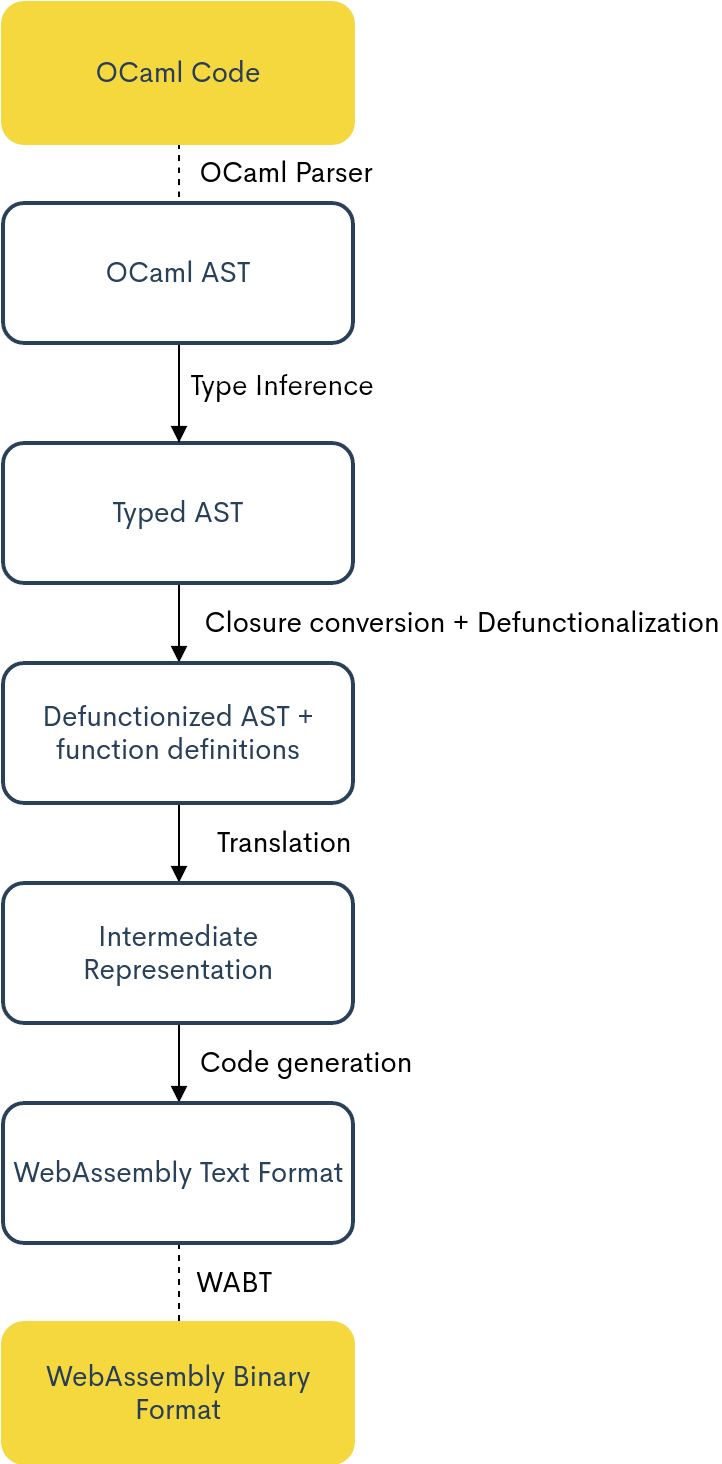
\includegraphics[width=0.55\linewidth]{otwa-diagram}
			\end{center}
		\end{columns}
	\end{frame}

	\begin{frame}
		\frametitle{What's Next}
		* Evaluation
		* Optimisations
		* More OCaml features
	\end{frame}
	
\end{document}
